\documentclass[12pt]{article}

\usepackage[margin=1in]{geometry}
\usepackage[T1]{fontenc}
\usepackage[utf8]{inputenc}
\usepackage{kotex}
\usepackage{graphicx}
\usepackage{underscore}
\usepackage[sort]{natbib}
\usepackage{booktabs}
\usepackage{amsmath}
\usepackage{subcaption}
\usepackage[hidelinks]{hyperref}
\usepackage{setspace}
\doublespacing

\graphicspath{{../output/figures/}}

\title{The Korea Discount: Corporate Governance Deficits, Structural Reform,\\and the Limits of Voluntary Intervention}
\author{Daniel Jung}
\date{May 8, 2026}

\begin{document}
\maketitle

\begin{abstract}
South Korean equities have traded at a structural discount to developed-market and emerging-market peers for over three decades. This paper does a review of 21 studies on the Korea Discount and presents original empirical evidence from a 20-year monthly panel of index-level price-to-book (P/B) ratios. The literature suggests three competing explanations---concentrated chaebol ownership and tunneling, weak minority shareholder protections, and stagnant growth fundamentals---but diverges on their relative importance. Cross-sectional regressions found formal governance scores insignificant once growth was controlled \citep{yang2025korea}, while natural experiments identified ownership-based self-dealing as a direct value destroyer \citep{black2015governance}. We examine this divergence using Japan's three governance reforms as a benchmark. A stacked event-study analysis shows that the 2014 Stewardship Code and 2015 Corporate Governance Code were not followed by any sustained re-rating, while the 2023 TSE P/B reform request coincided with a $-6.48$ P/B point cumulative KOSPI--TOPIX spread over 24 months, and the 2025 binding mandate coincided with further widening. Korea's 2024 Value-Up program, which remains voluntary, coincided with no improvement: MSCI EM Asia outperformed KOSPI by $+2.18$, $+1.80$, and $+2.12$ P/B points at $\tau=12$ across the three milestones. A geopolitical risk falsification also rejects acute geopolitical shocks as the driver of the discount ($t=-0.84$, $p=0.40$), but a structural level premium cannot be ruled out. The evidence seems to support enforceable reform over voluntary governance codes.
\end{abstract}

\section{Introduction}
\label{sec:intro}

The ``Korea Discount''---the persistent undervaluation of South Korean equities relative to global peers---is one of the most debated puzzles in international finance. Over 2004--2024, the KOSPI P/B ratio averaged $0.177\times$ below TOPIX ($t=-3.23$) and $0.601\times$ below MSCI EM ($t=-10.31$), with both gaps statistically significant under Newey-West HAC standard errors. The discount has persisted for at least three decades, widened after Japan's 2025 governance mandate, and resisted Korea's 2024 voluntary Value-Up program.

This paper makes two contributions. First, we synthesize 21 academic studies---including 11 published in Korean-language journals---organized around the competing explanations for the discount: governance and tunneling, growth fundamentals, and institutional stewardship. Second, we present original empirical evidence from a 20-year monthly panel covering KOSPI, TOPIX, S\&P~500, and MSCI~EM, using Japan's staged governance reforms as a policy benchmark. The central empirical pattern is that voluntary governance codes---whether Japan's 2014--2015 soft laws or Korea's 2024 Value-Up program---were not followed by sustained valuation improvement, while mandatory exchange-level enforcement with binding improvement plans and market-demotion consequences, as embodied in Japan's 2025 TSE P/B Mandate, was.

\section{Defining and Measuring the Discount}
\label{sec:measurement}

The Korea Discount refers to the chronic undervaluation of Korean equities as measured by below-peer price-to-book (P/B) and price-to-earnings (P/E) ratios. The most comprehensive international evidence documented persistently lower P/B and P/E multiples for Korean firms across 48 countries from 1990 to 2023, even after controlling for firm size, profitability, growth, GDP per capita, financial market development, and geopolitical risk \citep{kim2026korean}. The finding held across all sub-periods (1990s, 2000s, 2010s onward), demonstrating that the discount was structural, not cyclical.

Whether the discount reflects risk or mispricing is contested. Korean firms with book-to-market (BTM) ratios above one consistently outperformed lower-BTM firms. Furthermore, high BTM was associated with a higher probability of positive extreme returns and a lower probability of negative extremes, indicating mispricing rather than risk compensation \citep{jung2022korea}. A governance factor was the strongest cross-sectional predictor.

Figure~\ref{fig:pb_comparison} presents the 20-year P/B trajectory. Table~\ref{tab:summary_stats} reports the headline statistics. The KOSPI--TOPIX spread averages $-0.177\times$ (NW SE $= 0.055$, $t=-3.23$, 95\% CI: $[-0.284, -0.069]$); the KOSPI--MSCI EM spread averages $-0.601\times$ (NW SE $= 0.058$, $t=-10.31$, 95\% CI: $[-0.716, -0.486]$). The sub-period decomposition shows structural deterioration: the KOSPI--TOPIX gap widens from $0.05$ P/B points in 2004--2013 to $0.43$ points in 2023--2024. A sector-composition caveat applies: KOSPI is concentrated in cyclical hardware manufacturing (Samsung Electronics and SK Hynix alone account for roughly 30\% of index weight), while TOPIX and S\&P~500 carry larger shares of software, services, and consumer sectors that structurally command higher P/B multiples. \citet{kim2026korean} controls for firm-level characteristics across 48 countries and finds the discount survives, but the index-level spreads reported here do not adjust for sector weighting.

\begin{figure}[htbp]
    \centering
    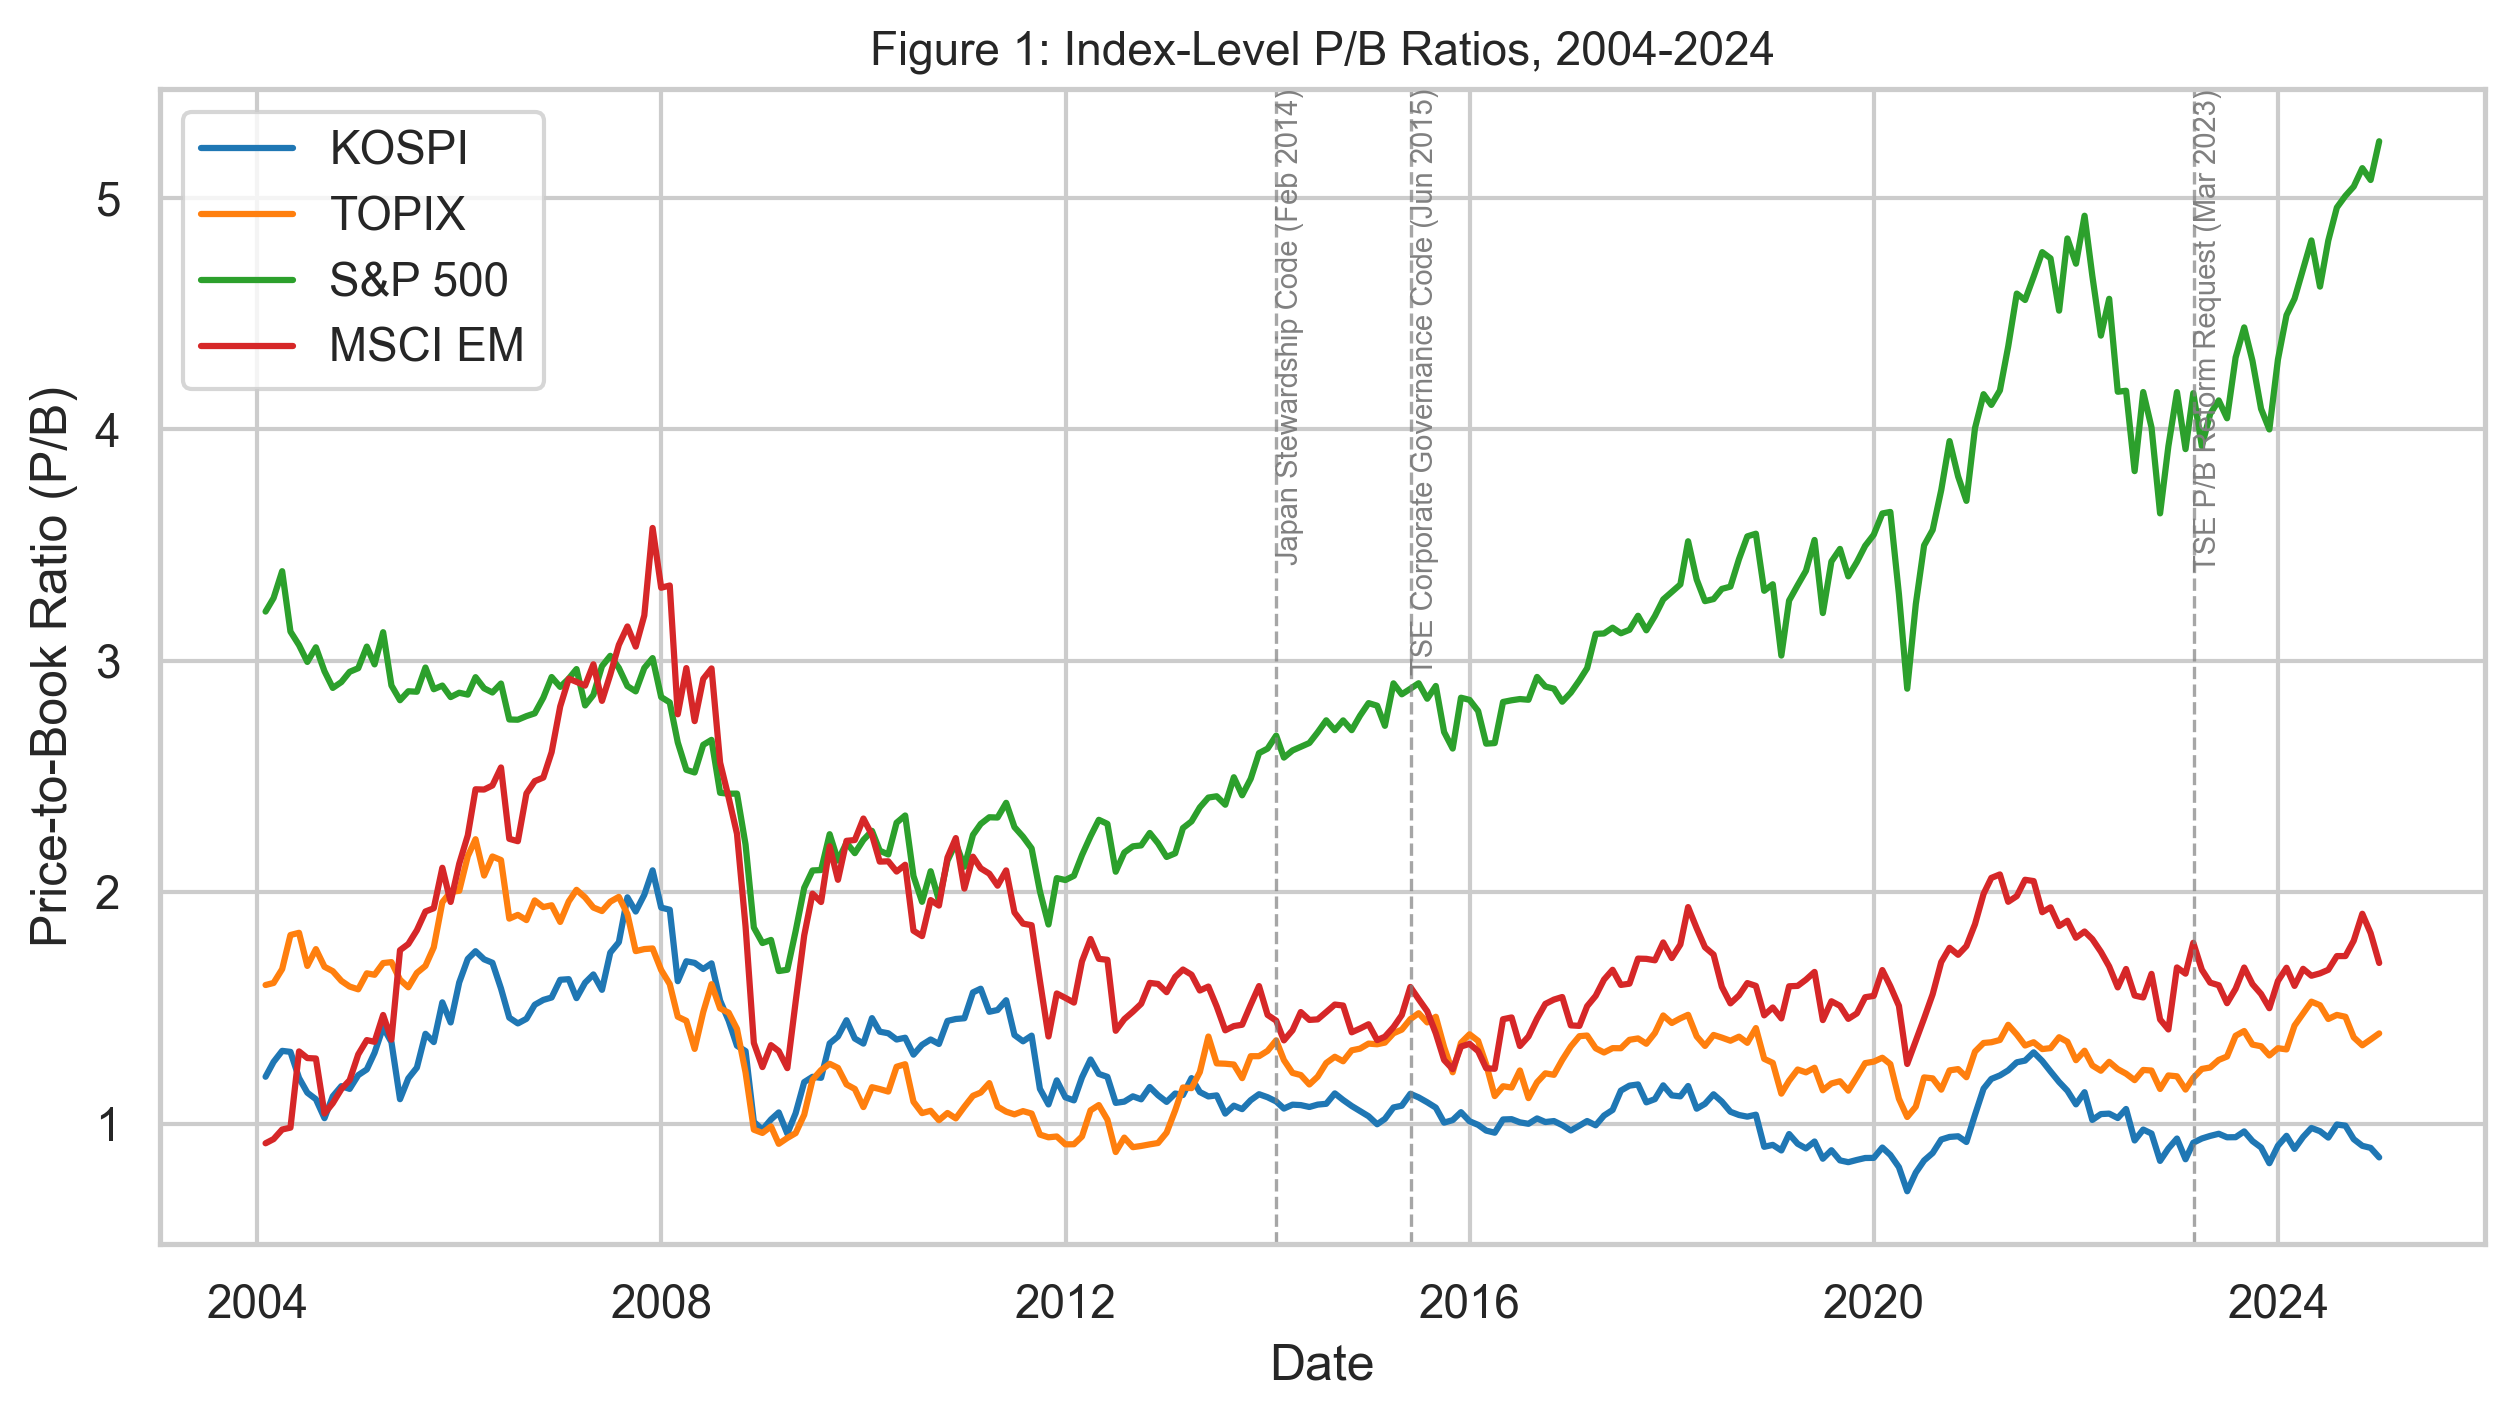
\includegraphics[width=0.95\textwidth]{figure1_pb_comparison.png}
    \caption{Monthly P/B ratios, January 2004--December 2024. Vertical lines mark Japan's governance reform milestones.}
    \label{fig:pb_comparison}
\end{figure}

\begin{table}
\caption{Summary statistics of index-level P/B ratios by country and sub-period.}
\label{tab:summary_stats}
\begin{tabular}{llrrrrr}
\toprule
 & Period & mean & median & std & min & max \\
country &  &  &  &  &  &  \\
\midrule
KOSPI & Full (2004--2024) & 1.18 & 1.10 & 0.26 & 0.71 & 2.09 \\
MSCI\_EM & Full (2004--2024) & 1.78 & 1.65 & 0.47 & 0.91 & 3.58 \\
SP500 & Full (2004--2024) & 3.08 & 2.89 & 0.81 & 1.66 & 5.25 \\
TOPIX & Full (2004--2024) & 1.35 & 1.31 & 0.28 & 0.88 & 2.23 \\
KOSPI & Pre-reform (2004--2013) & 1.36 & 1.34 & 0.25 & 0.96 & 2.09 \\
MSCI\_EM & Pre-reform (2004--2013) & 1.97 & 1.91 & 0.60 & 0.91 & 3.58 \\
SP500 & Pre-reform (2004--2013) & 2.51 & 2.42 & 0.40 & 1.66 & 3.39 \\
TOPIX & Pre-reform (2004--2013) & 1.41 & 1.29 & 0.39 & 0.88 & 2.23 \\
KOSPI & Reform era (2014--2022) & 1.02 & 1.03 & 0.12 & 0.71 & 1.31 \\
MSCI\_EM & Reform era (2014--2022) & 1.59 & 1.55 & 0.20 & 1.24 & 2.08 \\
SP500 & Reform era (2014--2022) & 3.39 & 3.28 & 0.63 & 2.58 & 4.92 \\
TOPIX & Reform era (2014--2022) & 1.29 & 1.28 & 0.10 & 1.03 & 1.48 \\
KOSPI & Post-TSE (2023--2024) & 0.93 & 0.94 & 0.04 & 0.83 & 1.00 \\
MSCI\_EM & Post-TSE (2023--2024) & 1.66 & 1.66 & 0.10 & 1.50 & 1.91 \\
SP500 & Post-TSE (2023--2024) & 4.51 & 4.47 & 0.43 & 3.91 & 5.25 \\
TOPIX & Post-TSE (2023--2024) & 1.36 & 1.35 & 0.10 & 1.15 & 1.53 \\
\bottomrule
\end{tabular}
\end{table}


\section{The Governance Channel: Chaebols, Tunneling, and Self-Dealing}
\label{sec:governance}

\subsection{Chaebol Ownership and Tunneling}

The structural foundation of the Korea Discount lies in Korea's chaebol system---family-controlled conglomerates that dominate the economy. Mapping chaebol formation revealed that controlling families used ``central firms'' to acquire low-profitability entities through pyramidal structures. These central firms traded at a discount, reflecting shareholders' anticipation of value-destroying acquisitions \citep{almeida2011chaebol}. 

The economic scale of tunneling was substantial: when a chaebol-affiliated firm made an acquisition, its stock price fell on average while the controlling shareholder benefited through value transfers to other group firms \citep{bae2002tunneling}. Business group-affiliated firms made systematically larger charitable donations. These donations were coordinated to tunnel resources from public affiliates (where families held lower cash flow rights) to private ones (where they held higher stakes) \citep{kim2019tunneling}.

The tunneling incentive is amplified by Korea's tax regime. South Korea imposes one of the highest statutory inheritance tax rates in the OECD---up to 60\% for controlling stakes in large firms---alongside dividends taxed as ordinary income at marginal rates up to 45\%. For controlling families whose wealth is concentrated in group equity, a higher share price directly increases succession-tax liability, creating a rational incentive to suppress valuations through low payouts, inter-affiliate transfers, and share-price discouragement. This tax structure makes tunneling not merely opportunistic but privately optimal: by keeping public-firm valuations depressed, controlling shareholders minimize both the fiscal cost of generational succession and the risk of losing control to hostile acquirers.

\subsection{Natural Experiment Evidence}

Exploiting Korea's 1999 reform that imposed stricter board requirements on large firms provides strong causal evidence. Event studies showed that large firms whose controllers had incentives to tunnel earned strong positive abnormal returns. Furthermore, panel regressions confirmed that better governance moderated the negative effect of related-party transactions on firm value and increased the sensitivity of firm profitability to industry profitability, consistent with reduced tunneling \citep{black2015governance}.

Concentrated ownership also distorts the broader governance environment. Among chaebol-affiliated firms, only shareholder rights protection retained explanatory power for dividend payouts; board effectiveness, audit competency, and disclosure transparency lost independent influence once ownership structure was controlled \citep{njoku2026governance}.

Another feature of chaebol conglomerates are their designated holding companies. Legally designated holding companies trade at significant P/B discounts relative to both operating companies and their fundamental values---a phenomenon unique to Korea and absent from Japan and the US \citep{park2019holding}. Cross-shareholding voting restrictions could positively influence capital markets by exposing holding companies to boardroom coups, inducing revaluation \citep{park2025cross}. However, this remains a defensive tactic rather than a fundamental governance improvement. Examining court rulings that weakened supermajority anti-takeover provisions showed that firms with such provisions outperformed, supporting their value-enhancing role when not abused for entrenchment \citep{kim2022supermajority}.

\section{The Growth vs.\ Governance Debate}
\label{sec:growth}

The tunneling and self-dealing evidence in Section~\ref{sec:governance} makes a strong case for governance as the primary driver of the discount, but there is a strand of cross-sectional literature that appears to contradict this.

Cross-sectional tests found that formal corporate governance scores had \emph{no} significant relationship with PBR. Stagnant growth variables instead dominated: low R\&D intensity, high tangible-asset intensity, and firm maturity all exhibited strong positive correlations with low PBR, while higher shareholder payouts were paradoxically associated with \emph{lower} PBR \citep{yang2025korea}. Large manufacturers corroborated this pattern---dividend expansion had weak or negative effects on PBR, and R\&D investment was the more significant predictor \citep{lee2025korea_pbr}. Across 58 markets from 2001 to 2018, Korea's formal shareholder rights scores were not distinctively low. What set Korea apart was low \emph{value relevance}: profitability and growth were incorporated into prices to a far lesser degree than in comparable markets (51st of 58 countries), pointing to a short-term investment culture that prevented long-term expectations from being capitalized \citep{kim2025causes}.

These findings are striking, but they test the wrong construct. The expropriation channel operates through the wedge between controlling families' voting rights and their economic stake---not through the board-composition and disclosure indices that governance scores measure. A chaebol can score adequately on formal metrics while simultaneously operating pyramidal structures that divert profits from public affiliates to private ones \citep{almeida2011chaebol}. Reducing family ownership concentration directly shrinks this wedge: as controlling shareholders capture a smaller share of private benefits, more earnings flow to minority shareholders, and P/B rises. This is a governance mechanism---a reduction in expropriation risk---that index scores are structurally ill-equipped to detect. The two channels plausibly reinforce one another. Controlling shareholders may prefer low-risk, tunnelable cash flows over long-horizon R\&D spending, causing governance-driven expropriation to register empirically as a growth deficit; low value relevance then weakens the market penalty for value-destroying acquisitions, further entrenching the cycle. While direct causal estimation of this feedback loop remains limited by endogeneity, the descriptive spread patterns in Section~\ref{sec:reform}---showing that spread widening coincided with enforceable reform milestones rather than with changes in growth fundamentals---are consistent with the governance channel as the deeper cause.

\section{Institutional Stewardship: Promises and Limits}
\label{sec:stewardship}

\subsection{NPS Activism}

Korea's first policy response leveraged the National Pension Service (NPS) as an activist institutional shareholder. However, markets did not react to NPS ``Vote No'' announcements, a result inconsistent with developed-market activism, though firms that subsequently improved internal governance showed higher valuations \citep{kim2014nps}. NPS shareholding improved ESG performance and financial outcomes, with ESG serving as the primary transmission channel \citep{kim2022nps_esg}. Furthermore, NPS ESG engagement disclosures were associated with significant firm value gains. These effects were strongest for firms with the weakest internal governance, indicating that institutional activism substituted for, rather than complemented, internal governance \citep{lee2026esg}.

\subsection{Stewardship Code and Foreign Investors}

Korea's 2016 Stewardship Code also asked institutional investors to adopt principles of responsible engagement---voting actively on shareholder resolutions, disclosing conflicts of interest, and monitoring investee companies---with the goal of improving corporate governance through investor pressure rather than legislative mandate. While a positive correlation was found between Stewardship Code adoption and earnings quality, multivariate regressions failed to establish statistical significance \citep{park2021stewardship}. The broader challenge was that Korea's formal governance scores were not distinctively lower than those of its peers; the problem lay in enforcement credibility rather than established norms \citep{kim2025causes}.

Foreign investors facilitated the incorporation of firm-specific information into stock prices more effectively than domestic institutions \citep{kim2015foreign}. Foreign ownership also reduced growth disparities through asymmetric discipline---correcting over-investment in over-growing firms and encouraging profitable management in under-growing ones. This implied that governance reforms that improved market accessibility could significantly amplify foreign investor discipline \citep{joo2026foreign}.

\section{Reform Benchmarks: Japan's Arc and Korea's Voluntary Response}
\label{sec:reform}

\subsection{Japan's Staged Governance Trajectory}

Japan faced a structurally similar valuation discount through the 2000s and 2010s, attributed to cross-shareholding (\textit{keiretsu}), weak board independence, and low dividend payouts. The government responded with three reforms escalating enforcement: (i) the Stewardship Code (February 2014), requiring institutional governance engagement; (ii) the Corporate Governance Code (June 2015), mandating board composition and disclosure standards; (iii) the TSE P/B Reform Request (March 2023), asking Prime Market firms below $1.0\times$ book value to disclose capital efficiency shortfalls and improvement plans---a comply-or-explain mandate: the TSE published monthly scorecards naming non-responsive firms, institutional investors used the lists in stewardship voting, and the Exchange signaled that compliance records would inform future market-classification reviews, producing near-universal engagement even without binding targets; and (iv) the TSE P/B Mandate (January 2025), requiring Prime Market firms below $1.0\times$ book value to submit binding, multi-year capital efficiency improvement plans with specific quantitative targets under threat of automatic demotion to the Standard Market.

\subsection{Korea's Value-Up Program}

Korea's 2024 Corporate Value-Up Program mirrors Japan's reform arc in aspiration but not in enforcement. Most listed companies ignored the voluntary guidelines, and the KOSPI closed weaker in 2024---the opposite outcome from Japan's experience following its 2023 TSE reform request. Evaluations of the program found low participation and weak market responses \citep{lee2025valueup}. Conversely, direct market evidence showed that \emph{legislative} reform shifted expectations: the 2025 Commercial Act amendment (which expanded directors' fiduciary duties to shareholders) produced significantly positive abnormal returns for high-book-to-market firms. There was no significant reaction among firms with high controlling-shareholder ownership, indicating that markets expected the reform to be most effective where expropriation risk was highest \citep{kang2026commercial}.

\subsection{Empirical Evidence: Japan Reform Benchmark}
\label{sec:empirical_japan}

We conducted stacked event studies \citep{cengiz2019} around Japan's three reform dates, using both a KOSPI--TOPIX spread (secondary) and an MSCI EM Asia--TOPIX spread (primary, insulating results from Japan-specific dynamics). Figure~\ref{fig:japan_es} presents the results. The cumulative abnormal spread (CAR) estimates below are descriptive: each accumulates the deviation of the actual spread from a pre-event linear trend extrapolation. No standard errors are reported---the saturated cohort $\times$ relative-time design makes robust inference undefined---so the figures illustrate the pattern of spread movements around each milestone rather than establishing causation. Confounders contemporaneous with each reform event, including Japan's broader macro re-rating in 2023--2025, cannot be ruled out.

\textbf{2014 Stewardship Code.} The MSCI EM Asia--TOPIX CAR reaches $+1.60$ at $\tau=20$---no sustained TOPIX re-rating. Korea did not underperform relative to trend.

\textbf{2015 Corporate Governance Code.} Qualitatively identical: KOSPI--TOPIX CAR $+7.83$ at $\tau=24$; Asia CAR $+1.60$ at $\tau=20$. Neither soft-law event was followed by a sustained shift in the spread.

\textbf{2023 TSE P/B Reform Request.} The spread pattern in the months following this event is markedly different. The KOSPI--TOPIX cumulative spread declines to $-6.48$ at $\tau=24$; the MSCI EM Asia--TOPIX cumulative spread reaches $-2.58$ at $\tau=20$---the largest spread movement in the sample.

\begin{figure}[htbp]
    \centering
    \begin{subfigure}[b]{0.49\textwidth}
        \centering
        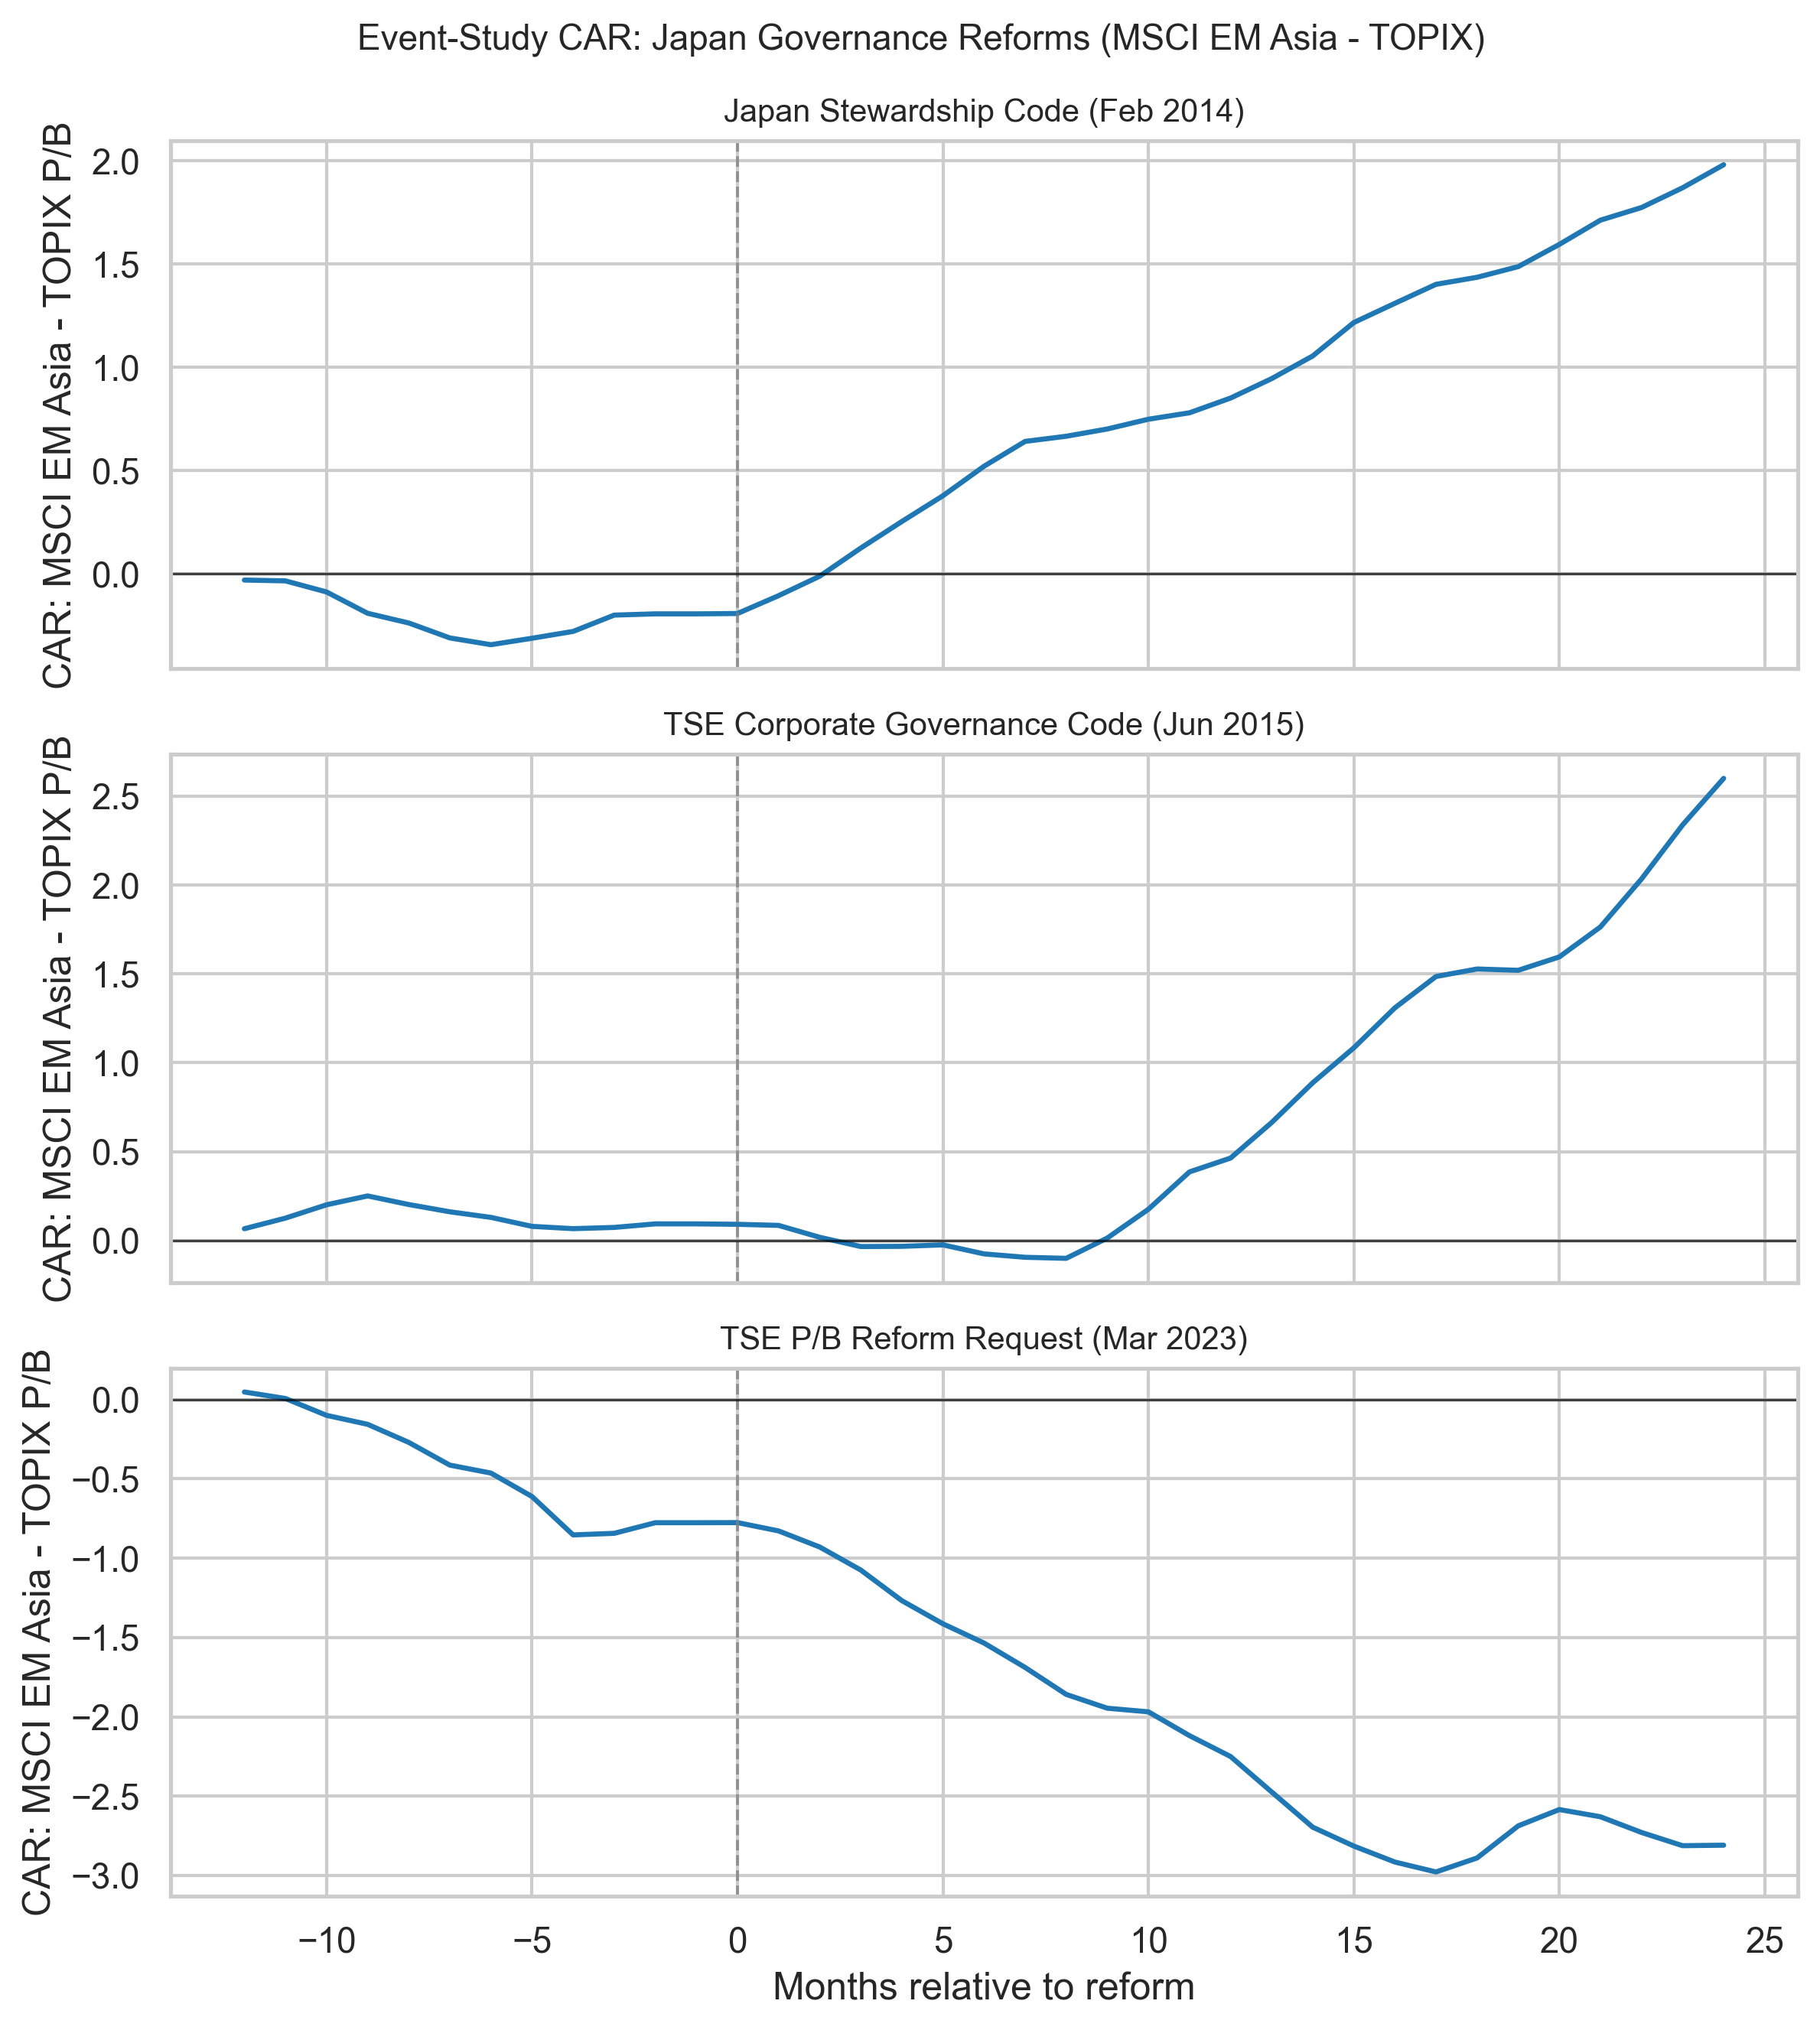
\includegraphics[width=\textwidth]{figure_asia_event_study.png}
        \caption{MSCI EM Asia--TOPIX}
    \end{subfigure}
    \hfill
    \begin{subfigure}[b]{0.49\textwidth}
        \centering
        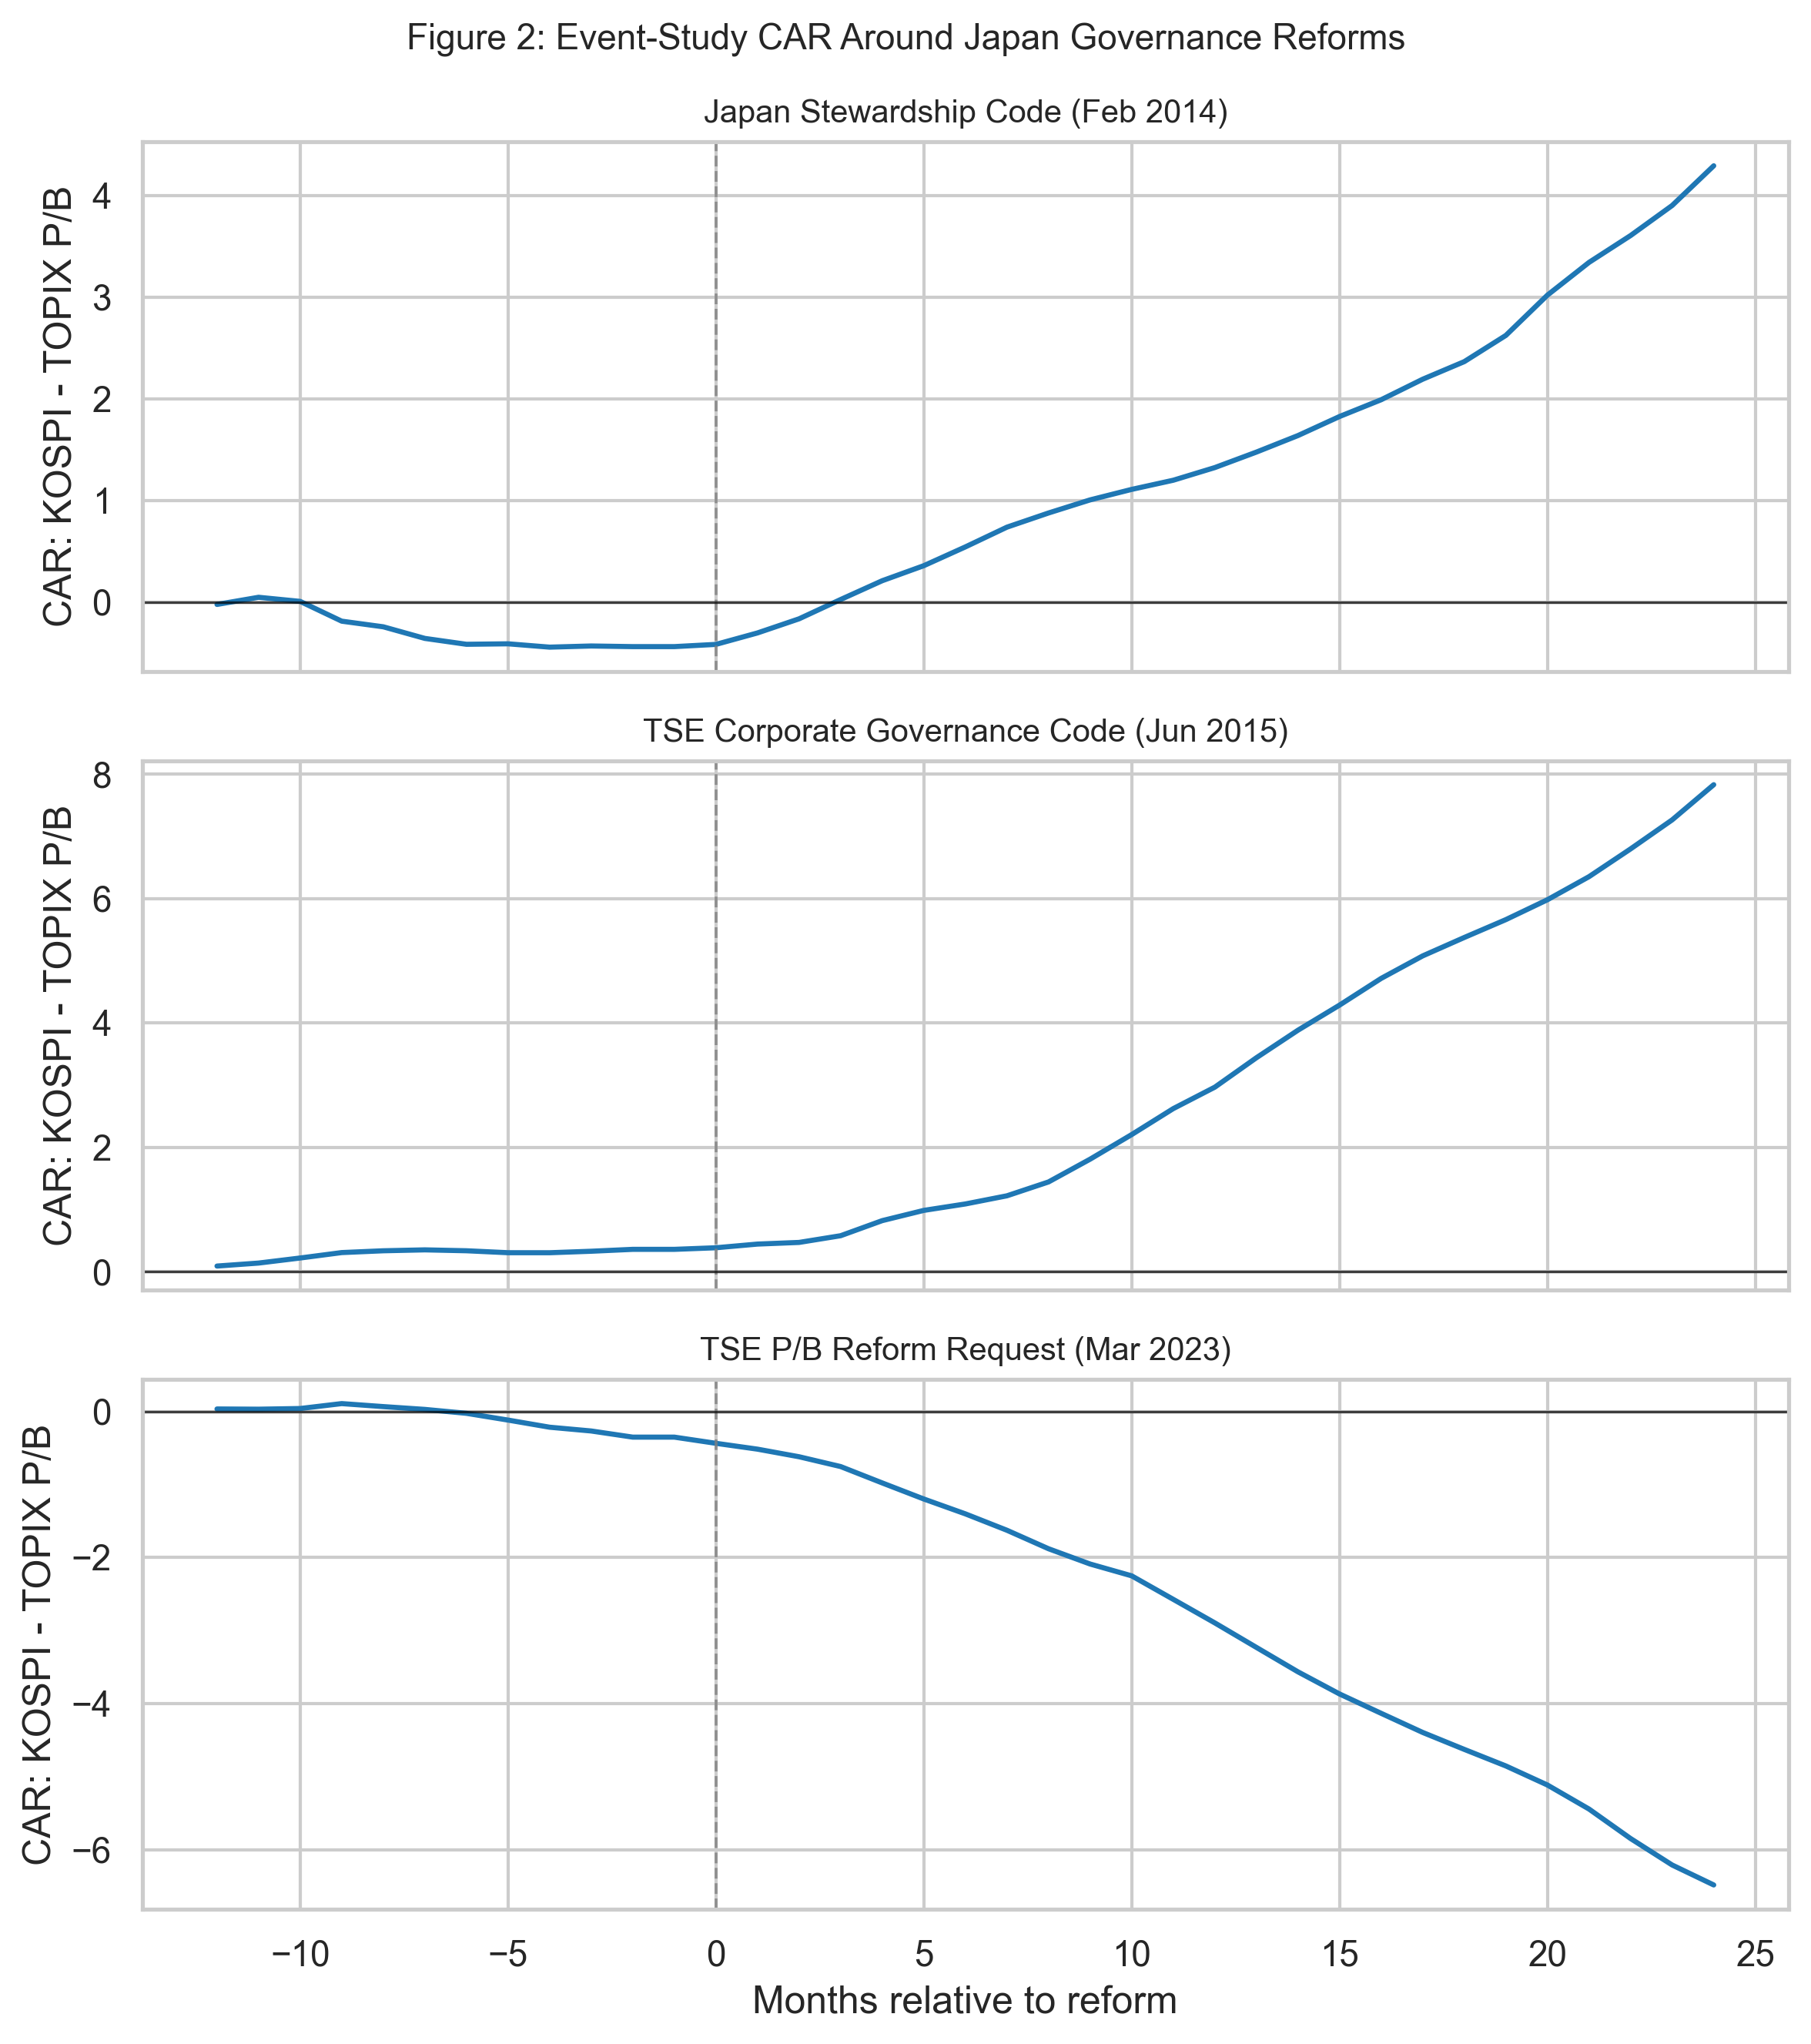
\includegraphics[width=\textwidth]{figure2_event_study.png}
        \caption{KOSPI--TOPIX}
    \end{subfigure}
    \caption{Japan governance reform event studies. The 2023 TSE P/B reform request is followed by a $-6.48$ P/B point KOSPI--TOPIX cumulative spread, while the 2014 and 2015 soft codes are not followed by any sustained spread shift.}
    \label{fig:japan_es}
\end{figure}

Figure~\ref{fig:japan_followon} extends the window through the 2025 TSE binding mandate. The KOSPI--TOPIX spread widens beyond the $-6.48$ P/B point mark established at $\tau=24$ under the reform request, consistent with the illustrative pattern that greater enforcement stringency accompanies larger spread movements.

\begin{figure}[htbp]
    \centering
    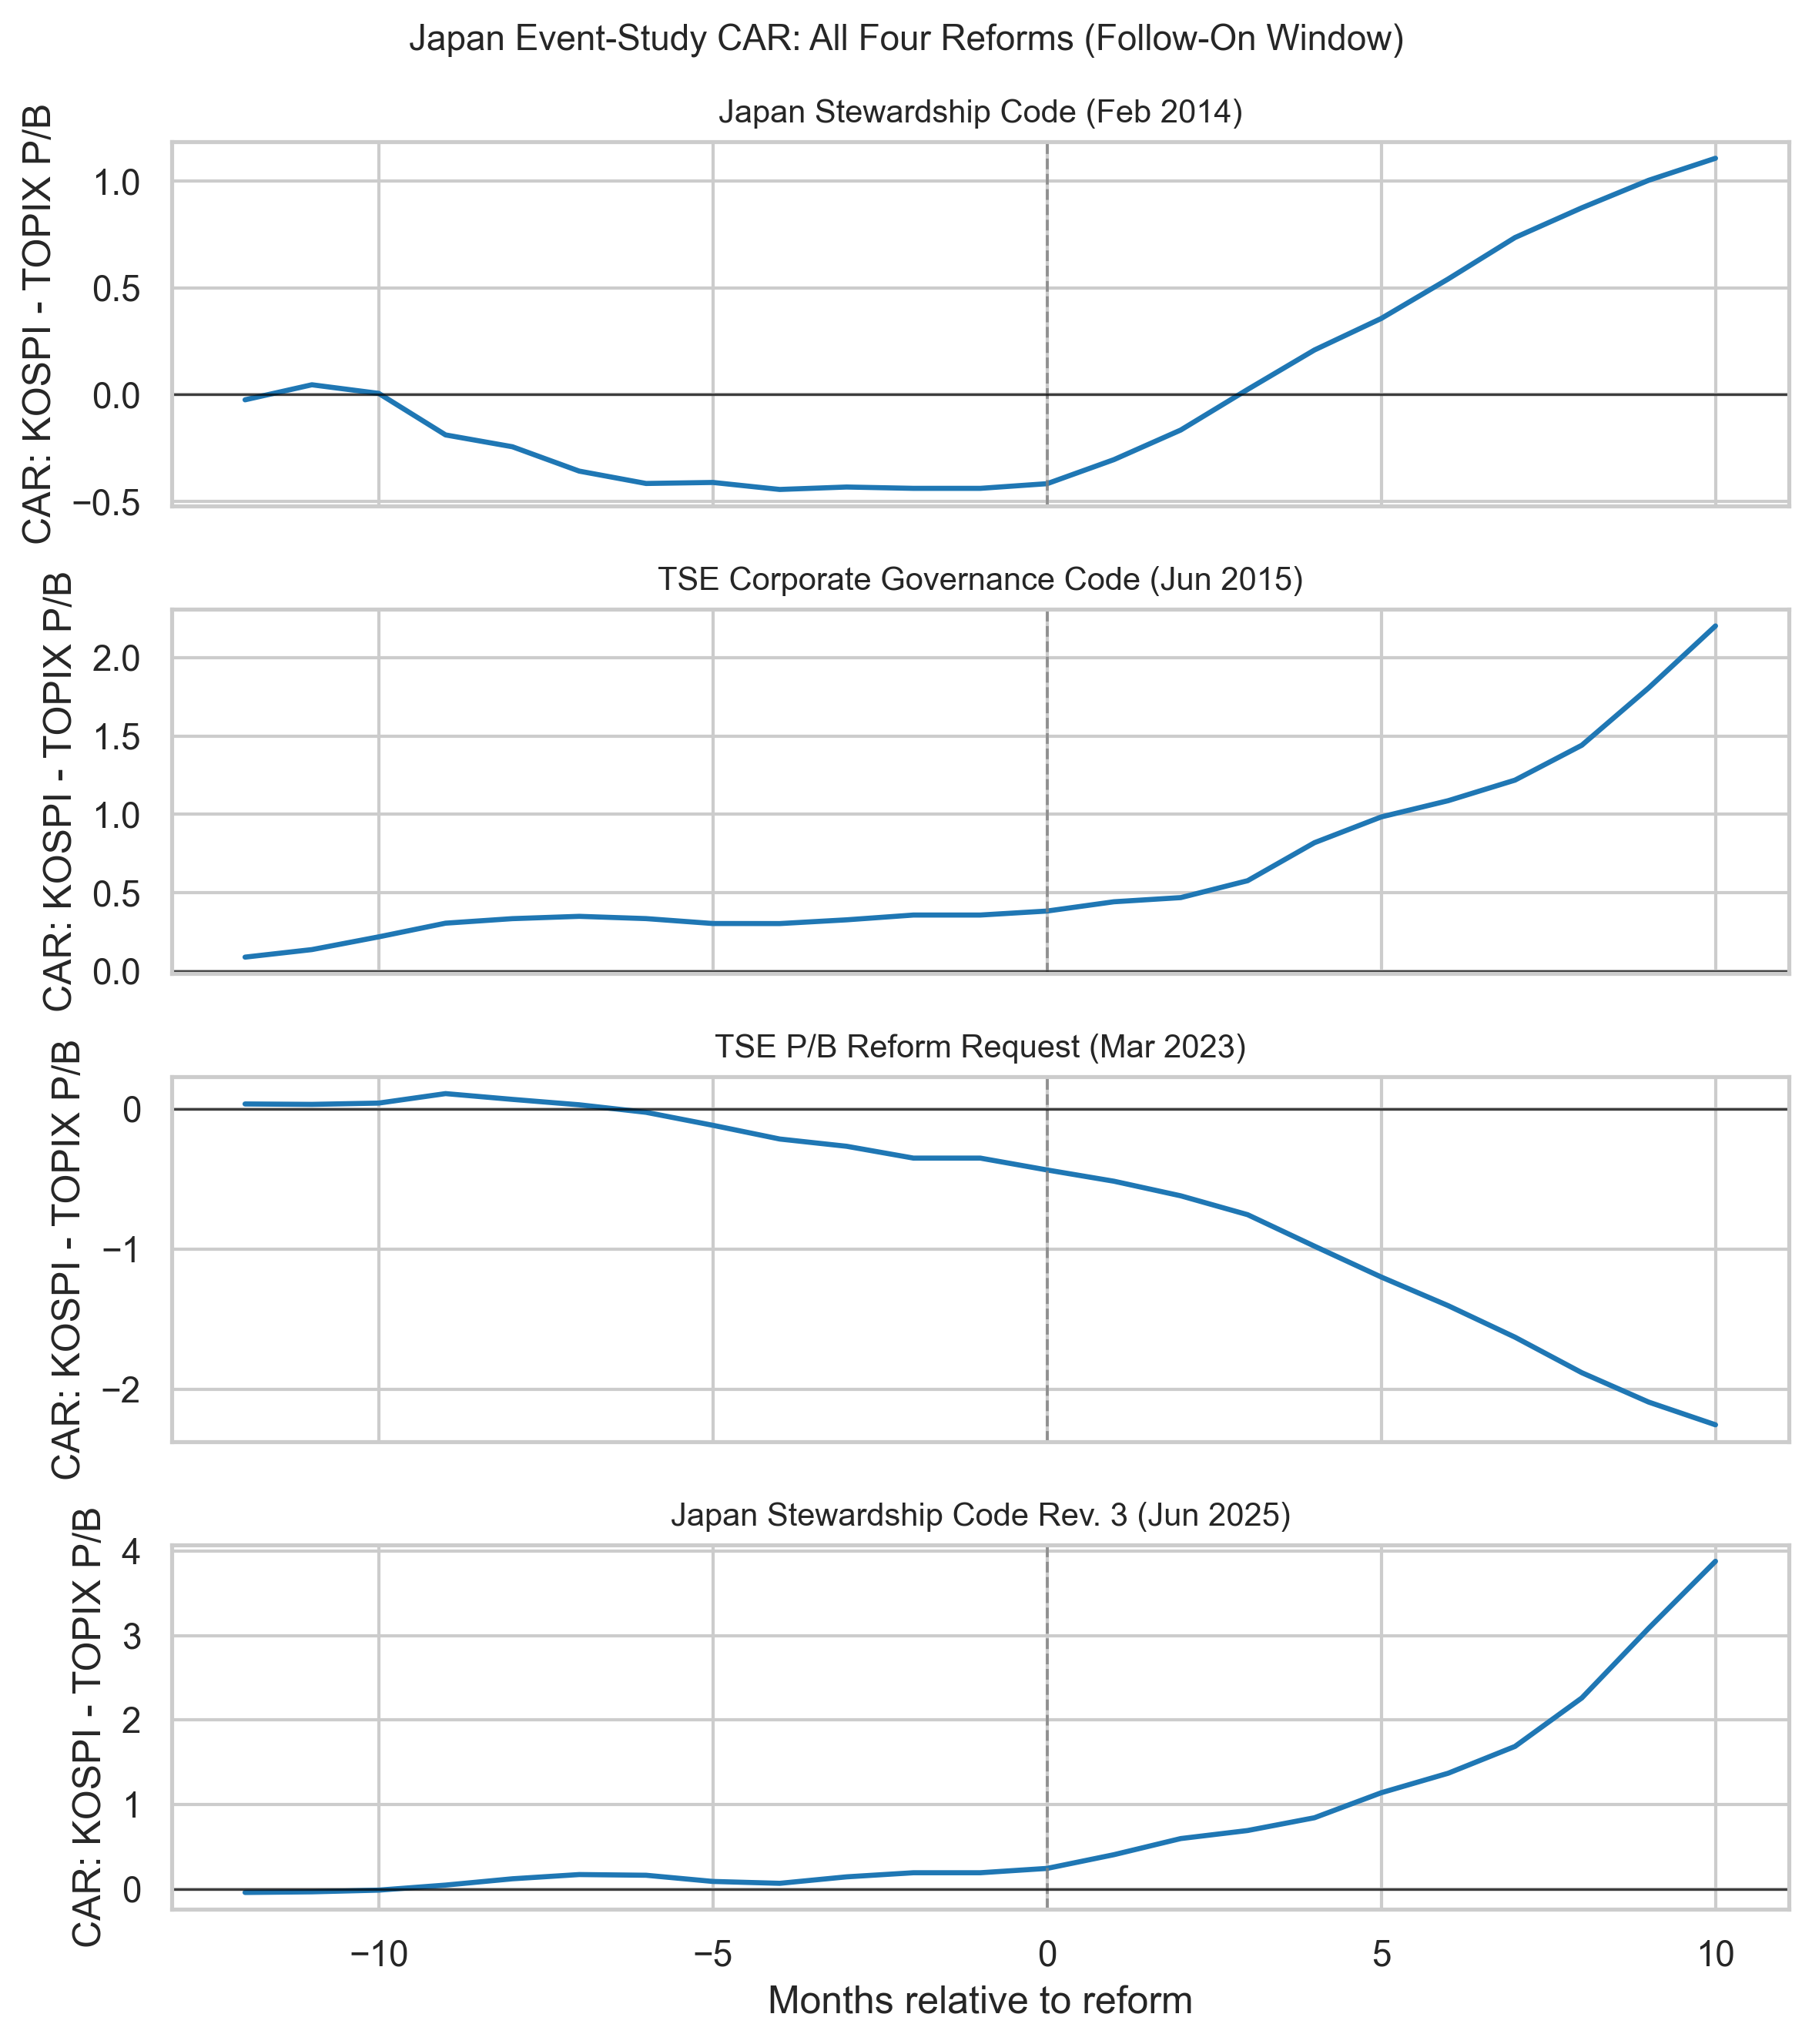
\includegraphics[width=0.95\textwidth]{figure_japan_follow_on_event_study.png}
    \caption{Japan follow-on event study: 2025 TSE binding mandate extension. The KOSPI--TOPIX spread widens beyond the $-6.48$ P/B point cumulative spread established in the 2023 reform request window, consistent with the pattern that greater enforcement stringency accompanies larger spread movements.}
    \label{fig:japan_followon}
\end{figure}

\subsection{Empirical Evidence: Korea's Value-Up Program}

Figure~\ref{fig:korea_es} presents the Korea Value-Up event study. Both spreads---MSCI EM Asia minus KOSPI and TOPIX minus KOSPI---are persistently positive at all three milestones, meaning both benchmarks outperformed KOSPI throughout. For the program launch (February 2024): MSCI EM Asia--KOSPI CAR $+2.18$ at $\tau=12$ and $+4.14$ at $\tau=20$. For the guidelines unveiling (May 2024): $+1.80$ at $\tau=12$. For the implementation push (August 2024): $+2.12$ at $\tau=12$. Korea's voluntary program coincided with no improvement in relative valuation.

\begin{figure}[htbp]
    \centering
    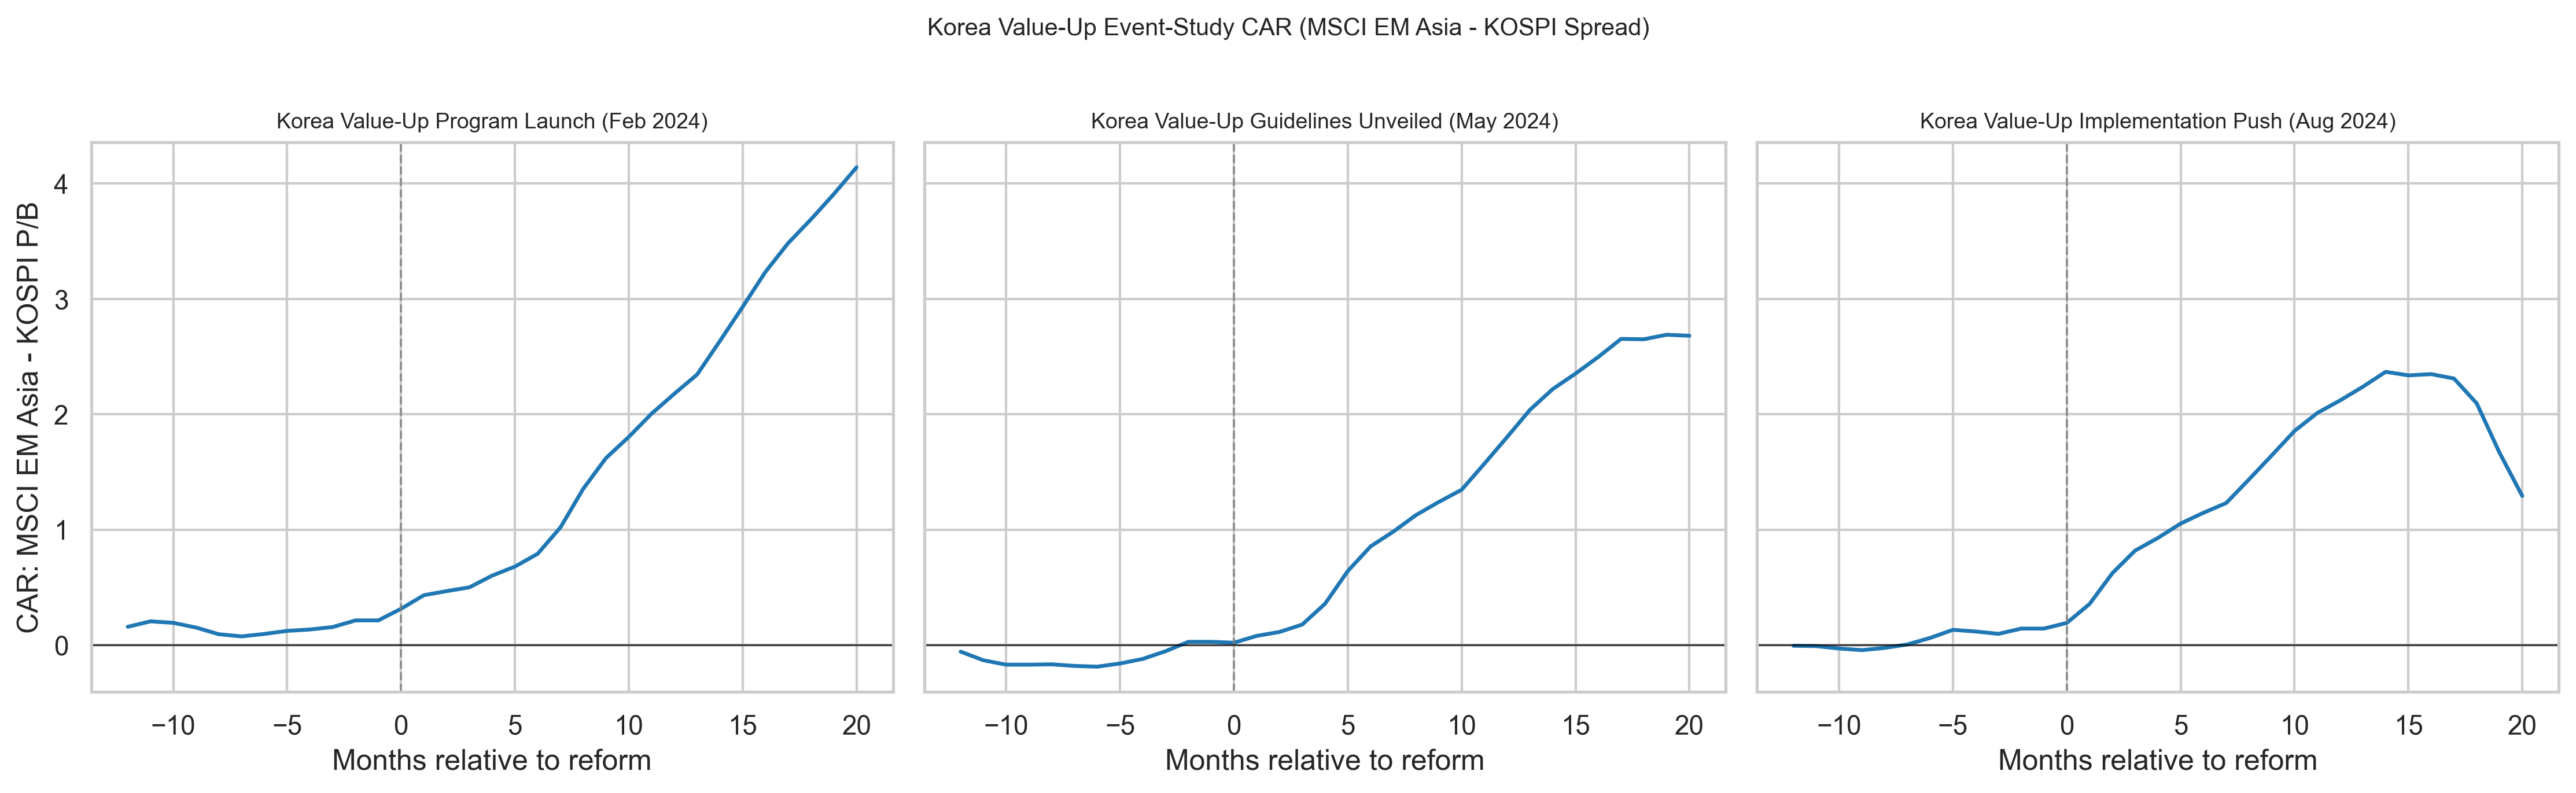
\includegraphics[width=0.95\textwidth]{figure_korea_asia_event_study.png}
    \caption{Korea Value-Up event study (MSCI EM Asia--KOSPI). All three milestones are followed by persistently positive cumulative spreads, with MSCI EM Asia outperforming KOSPI throughout.}
    \label{fig:korea_es}
\end{figure}

\section{Geopolitical Risk and Other Explanations}
\label{sec:geopolitical}

North Korean geopolitical risk is the most frequently invoked lay explanation for the Korea Discount, but the empirical record provides limited support for it. The theoretical intuition---that proximity to an unpredictable nuclear-armed state raises the equity risk premium and depresses valuations---is plausible in isolation. In practice, however, North Korean provocations are too predictable in their repetition and too limited in their macroeconomic consequences for markets to price them as incremental uncertainty. Cross-country studies that directly control for geopolitical risk find the discount survives fully intact \citep{kim2026korean}: markets appear to treat North Korean threats as a chronic, long-since-priced background condition. When researchers decompose cross-country discount differentials, it is Korea's economic policy uncertainty index---not military threat---that provides explanatory power \citep{kim2025causes}.

\subsection{Geopolitical Risk Falsification}

To formalize the test, we regress KOSPI P/B on a Korea GPR escalation dummy (GPRC\_KOR, \citealt{caldara2022}, above its 75th percentile), controlling for TOPIX P/B and year fixed effects over 252 monthly observations (January 2004--December 2024). The GPR coefficient is $-0.016$ ($t=-0.84$, $p=0.40$)---statistically indistinguishable from zero and economically negligible at less than one-tenth of the mean KOSPI--TOPIX spread. The specification is biased toward finding an effect, since GPRC\_KOR may also capture global risk-off episodes that depress Korean valuations for non-geopolitical reasons; it still finds none. Figure~\ref{fig:geo_risk} presents the KOSPI P/B series alongside GPR escalation episodes; no systematic co-movement is apparent even around the most acute crises.

\begin{figure}[htbp]
    \centering
    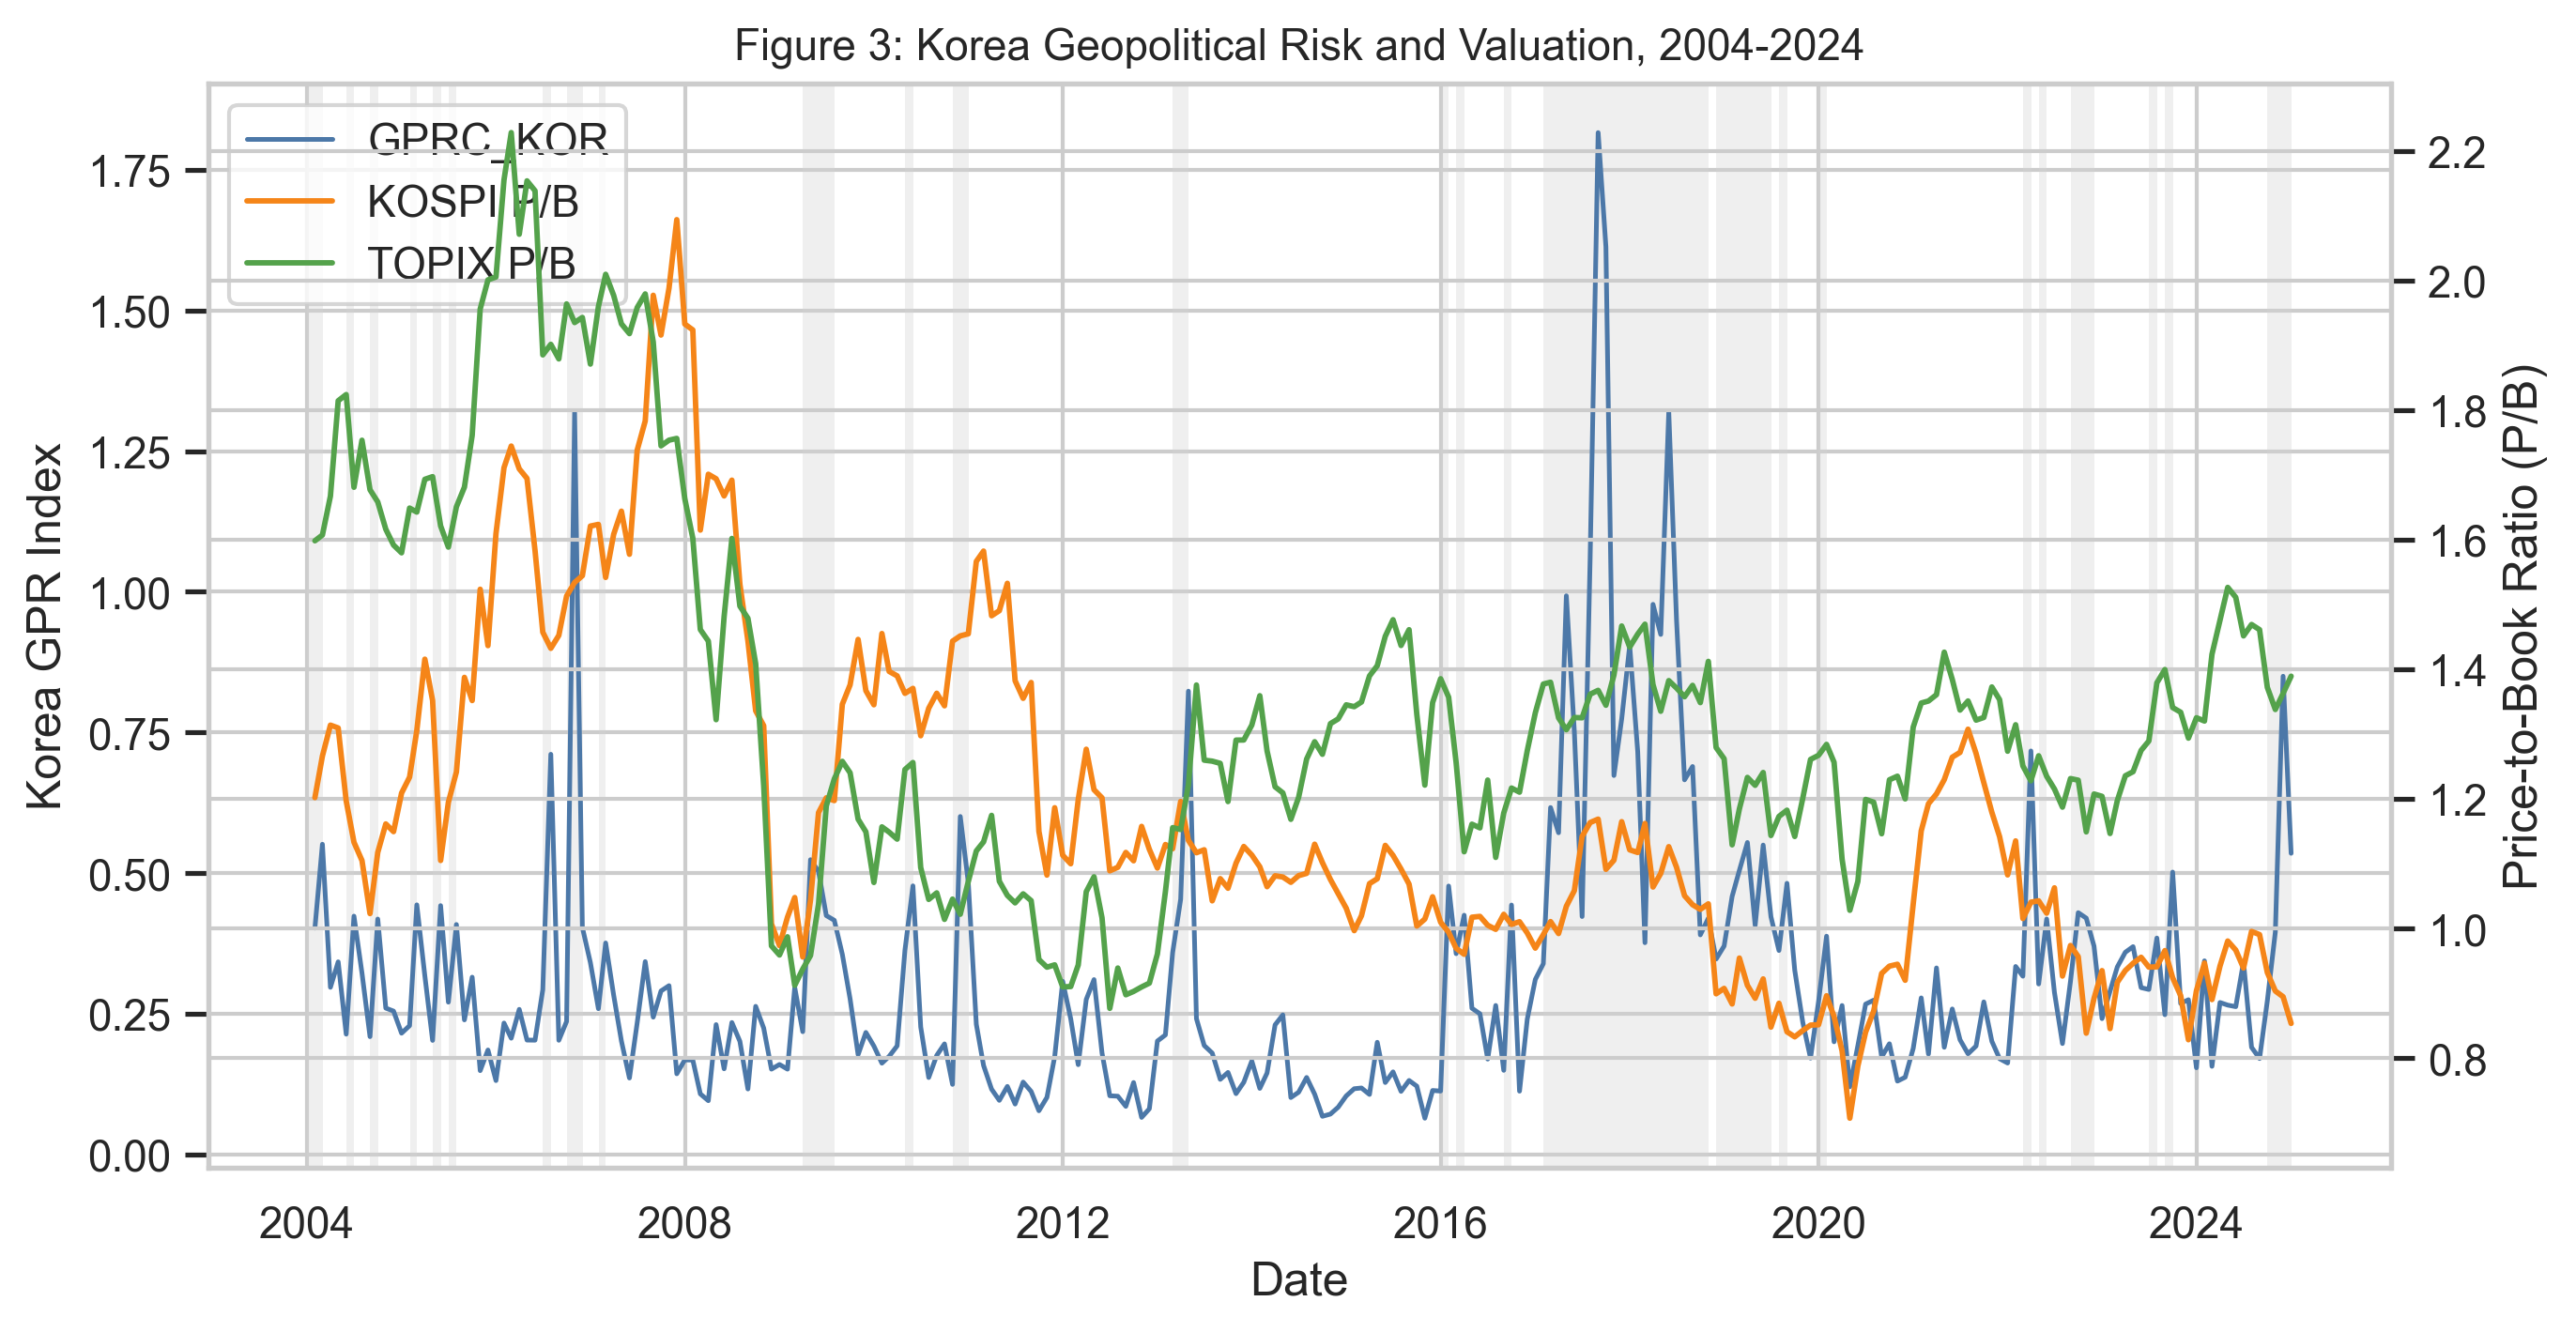
\includegraphics[width=0.95\textwidth]{figure3_geo_risk.png}
    \caption{KOSPI P/B and North Korea geopolitical risk escalation episodes. Shaded regions mark periods when the Korea GPR index (GPRC\_KOR) exceeded its 75th percentile. No systematic co-movement is apparent; the regression coefficient is $-0.016$ ($t=-0.84$, $p=0.40$).}
    \label{fig:geo_risk}
\end{figure}

\section{Synthesis and Policy Implications}
\label{sec:synthesis}

The literature and empirical evidence suggest mitigating the Korea Discount requires enforceable reform with credible sanctions, not voluntary guidelines.

The central empirical pattern in this paper is the three-step escalation of Japan's governance reforms. Japan's 2014 and 2015 voluntary codes were not followed by any sustained TOPIX re-rating. The 2023 TSE P/B reform request---still formally voluntary but backed by monthly public compliance scorecards and implicit reclassification pressure---coincided with a $-6.48$ P/B point KOSPI--TOPIX cumulative spread over 24 months. The 2025 binding mandate with automatic demotion coincided with further spread widening (Figure~\ref{fig:japan_followon}). Each step toward binding enforcement was accompanied by a larger spread movement in the data. Korea's 2024 voluntary Value-Up program saw MSCI EM Asia outperform KOSPI at all three milestones, with persistently positive MSCI EM Asia--KOSPI cumulative spreads (Figure~\ref{fig:korea_es}).

Institutional stewardship through the NPS has produced conditional improvements \citep{kim2022nps_esg, lee2026esg}, but markets did not react to NPS vote-no announcements \citep{kim2014nps} and stewardship code adoption failed to reach statistical significance in multivariate tests \citep{park2021stewardship}. (This is consistent with the broader pattern that voluntary engagement lacks enforcement credibility without structural reform.) Foreign investor discipline offers a complementary channel \citep{joo2026foreign, kim2015foreign}, but its efficacy depends on market accessibility reforms that increase foreign ownership. The geopolitical risk alternative also has no credibility: the Korea GPR coefficient is $-0.016$ ($t=-0.84$, $p=0.40$), economically negligible and statistically indistinguishable from zero.

Korea's 2025 Commercial Act amendment, which expanded directors' fiduciary duties to shareholders, produced significant positive abnormal returns for high-discount firms \citep{kang2026commercial}---validating the hard-law mechanism and representing a genuine step forward. But its fiduciary duty expansion operates through litigation, whereas Japan's TSE mandate operates at the exchange level. Two confounds complicate reading the current spread. The global semiconductor boom produced outsized equity gains in both Korea (SK Hynix, Samsung Electronics) and Taiwan (TSMC), compressing the KOSPI gap to peers through a cyclical channel independent of governance reform; any near-term Korea re-rating should be interpreted with that caveat. At the same time, TOPIX has reached all-time highs in 2025-2026, breaking through levels last seen at Japan's 1989 bubble peak and closing out the lost decades. That the reform sequence documented here coincides with TOPIX's historic recovery is consistent with the illustrative spread patterns in the event studies, though the same coincidence underscores the identification challenge: TOPIX's historic rise reflects a confluence of governance reform, yen depreciation, foreign capital reentry, and domestic demand recovery that the descriptive spread estimates alone cannot disentangle. Whether Korea's 2025 Commercial Act produces a comparable re-rating will become clearer as the semiconductor cycle matures.

{\singlespacing
\bibliographystyle{plainnat}
\bibliography{references}
}

\begin{center}
    "I pledge my honor that I have not violated the honor code during this assignment."\\
    \vspace{0.5cm}
    \textbf{Daniel Jung}
\end{center}

\end{document}